\chapter{String}

\section{Palindrome}
\subsection{Palindrome anagram}
\runinhead{Test palindrome anagram.} Char counter, number of odd count should $\leq 0$.
\runinhead{Count palindrome anagram.} See Section-\ref{N_objects_K_types}.
\runinhead{Construct palindrome anagram.} Construct all palindrome anagrams given a string \pyinline{s}.
\\
Clues:
\begin{enumerate}
\item dfs, grow the counter map of \pyinline{s}. 
\item jump parent char
\end{enumerate}
Code:
\begin{python}
def grow(self, s, count_map, pi, cur, ret):
  if len(cur) == len(s):
    ret.append(cur)
    return

  for k in count_map.keys():
    if k != pi and count_map[k] > 0:
      # jump the parent
      for i in xrange(1, count_map[k]/2+1):
        count_map[k] -= i*2
        self.grow(s, count_map, k, k*i+cur+k*i, ret)
        count_map[k] += i*2
\end{python}


\section{KMP}
Find string $W$ in string $S$ within complexity of $O(|W|+|S|)$.
\subsection{Prefix suffix table}
Partial match table (also known as "failure function"). After a failure matching, you know that the matched suffix before the failure point is already matched; therefore when you shift the $W$, you only need to shift the prefix onto the position of the previous suffix. The prefix and suffix must be proper prefix and suffix.

\begin{figure}[hbtp]
\centering
\subfloat{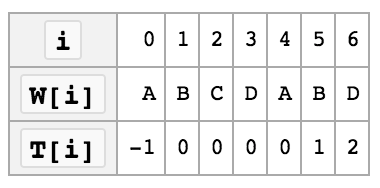
\includegraphics[scale=1.30]{kmp_table}}
\caption{Prefix-suffix table}
\label{fig:kmp_table}
\end{figure}
In table-building algorithm, similar to dp, let $T[i]$ store the length of matched prefix suffix for $needle[:i]$\\
\\
Clues:
\begin{enumerate}
\item dummy at $T[0]=-1$.
\item three parts
\begin{enumerate}
\item matched
\item fall back (consider $ABABC...ABABA$)
\item restart 
\end{enumerate}
\end{enumerate}
Table-building code:
\begin{python}
# construct T
T = [0 for _ in xrange(len(needle)+1)]
T[0] = -1
T[1] = 0

cnd = 0  
i = 2  # table index
while i < len(needle)+1:
    if needle[i-1] == needle[cnd]:  # matched
        T[i] = cnd+1
        cnd += 1
        i += 1
    elif T[cnd] != -1:  # fall back 
        cnd = T[cnd]
    else:  # restart 
        T[i] = 0
        cnd = 0
        i += 1
\end{python}
\subsection{Searching algorithm}
\begin{figure}[F]
\centering
\subfloat{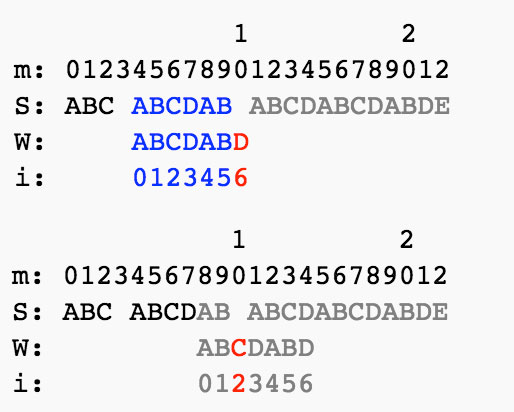
\includegraphics[scale=1.30]{kmp_presuffix}}
\caption{KMP example}
\label{fig:kmp_presuffix}
\end{figure}

Notice:
\begin{enumerate}
\item index $i$ and $j$.
\item $T[i-1+1]$ for corresponding previous index in $T$ for current scanning index $i$. 
\item When falling back, the next scanning index is \pyinline{len(prefix)}
\item three parts:
\begin{enumerate}
\item matched
\item aggressive move and fall back
\item restart 
\end{enumerate}
\end{enumerate}
Search code: 
\begin{python}
# search
i = 0  # index for needle 
j = 0  # index for haystack
while j+i < len(haystack):
    if needle[i] == haystack[j+i]:  # matched 
        i += 1
        if i == len(needle):
            return haystack[j:]
    else:
        if T[i] != -1:  # move and fall back j
            j = j+i-T[i]
            i = T[i]
        else:  # restart
            j += 1
            i = 0

return None
\end{python}
\subsection{Applications}
\begin{enumerate}
\item Find needle in haystack. 
\item Shortest palindrome 
\end{enumerate}

